%! TeX program = lualatex
\documentclass[a4paper]{article} 

% packages
\usepackage{microtype}      % Slightly tweak font spacing for aesthetics
\usepackage[english]{babel} % Language hyphenation and typographical rules
\usepackage[final, colorlinks = true, urlcolor = black, linkcolor = black]{hyperref} 
\usepackage{changepage}     % adjust margins on the fly

\usepackage{fontspec}
\setmainfont{EB Garamond}
\setmonofont[Scale=MatchLowercase]{Deja Vu Sans Mono}

\usepackage{minted}
\usemintedstyle{algol_nu}
\usepackage{xcolor}

\usepackage{pgfplots}
\pgfplotsset{width=\textwidth,compat=1.9}

\usepackage{caption}
\newenvironment{code}{\captionsetup{type=listing}}{}
\captionsetup[listing]{skip=0pt}
\setlength{\abovecaptionskip}{5pt}
\setlength{\belowcaptionskip}{5pt}

\usepackage[yyyymmdd]{datetime}
\renewcommand{\dateseparator}{--}

\usepackage{titlesec}
% \titleformat{\section}{\LARGE\bfseries}{}{}{}[\titlerule]
% \titleformat{\subsection}{\Large\bfseries}{}{0em}{}
% \titlespacing{\subsection}{0em}{-0.7em}{0em}
%
% \titleformat{\subsubsection}{\large\bfseries}{}{0em}{$\bullet$ }
% \titlespacing{\subsubsection}{1em}{-0.7em}{0em}

% margins
\addtolength{\hoffset}{-2.25cm}
\addtolength{\textwidth}{4.5cm}
\addtolength{\voffset}{-3.25cm}
\addtolength{\textheight}{5cm}
\setlength{\parskip}{0pt}
\setlength{\parindent}{0in}
% \setcounter{secnumdepth}{0}

\begin{document}
\hrule \medskip
\begin{minipage}{0.295\textwidth} 
    \raggedright
    \footnotesize 
    \begin{tabular}{@{}l l}
        Name: & Andrew Hayes \\
        Student ID: & 21321503 \\
        E-mail: & \href{mailto://a.hayes18@universityofgalway.ie}{\texttt{a.hayes18@universityofgalway.ie}} \\
    \end{tabular}
\end{minipage}
\begin{minipage}{0.4\textwidth} 
    \centering 
    \vspace{0.4em}
    \LARGE
    \textsc{ct420} \\ 
\end{minipage}
\begin{minipage}{0.295\textwidth} 
    \raggedleft
    \today
\end{minipage}
\medskip\hrule 
\begin{center}
    \normalsize
    Assignment 1: NTP Benchmarking
\end{center}
\hrule
\medskip

\section{NTP Installation}
As I already use a Linux-based operating system on my personal laptop, I first attempted to run \mintinline{shell}{ntpq} without installing anything, assuming it would be installed;
to my surprise, Arch Linux is so minimalist that it doesn't even come with the \mintinline{shell}{ntpd} package by default and I had to install it myself!
That explains why my system clock has always been two minutes behind for the past few years!
After installing \mintinline{shell}{ntpd} and enabling the daemon, and watching my system clock slowly speed up until it matched UTC, I checked that it was working properly by running \mintinline{shell}{ntpq -p} a few times:

\begin{figure}[H]
    \centering
    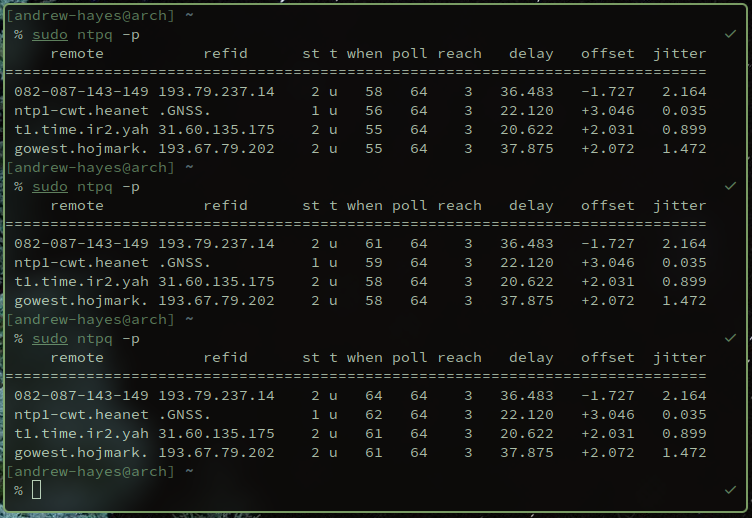
\includegraphics[width=\textwidth]{./images/ntpq-p.png}
    \caption{Verifying that the NTP daemon is running, via \mintinline{shell}{ntpq}}
\end{figure}

\section{NTP Configuration}
To select my servers in different locations for this assignment, I went through the pools for each location on \url{https://www.ntppool.org/} and added each one to my \verb|/etc/ntpc.conf| file one at a time, removing all other servers from the configuration file each time.
Then, I restarted the \verb|ntpd| service by running \mintinline{shell}{sudo systemctl restart ntpd}.
Finally, I ran \mintinline{shell}{ntpq -p} and picked a \verb|remote| for each area at random.

\begin{code}
\begin{minted}[linenos, breaklines, frame=single]{shell}
server bray.walcz.net   # Ireland
server 213.5.132.231    # United Kingdom
server 150.241.82.187   # Europe (Sweden)
server arm1.maxhost.io  # United States
server 159.196.178.7    # Australia
server 202.65.114.202   # Asia (Indonesia)
\end{minted}
\caption{Servers added to \texttt{/etc/ntp.conf}}
\end{code}

\begin{figure}[H]
    \centering
    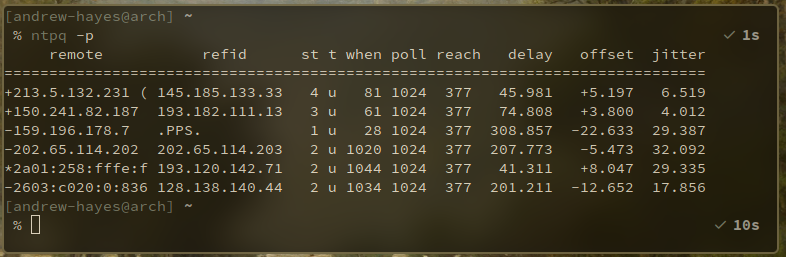
\includegraphics[width=\textwidth]{./images/ntpqoutput.png}
    \caption{Output of \texttt{ntpq -p} with new servers added}
\end{figure}

\subsection{Ireland Server}
The Ireland server I added had \verb|remote| \verb|bray.walcz.net| and appeared in the \verb|nptq -p| output with \verb|remote| \verb|2a01:258:fffe:f| which is just an abbreviated form of the IPv6 address \verb|2a01:258:fffe:f800:0:0:0:1|.

\begin{figure}[H]
    \centering
    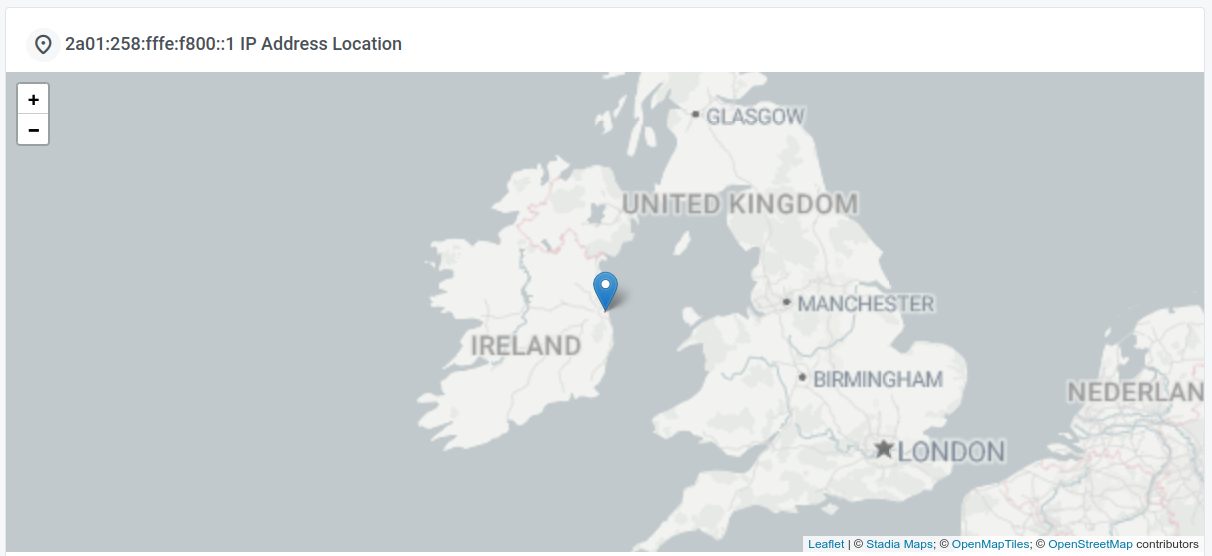
\includegraphics[width=\textwidth]{./images/irelandserverloc.png}
    \caption{Location of my chosen Ireland server (source: \url{https://www.ipaddress.com/})}
\end{figure}

According to \url{https://gps-coordinates.org/distance-between-coordinates.php} the distance between the latitude and longitude of Galway (as given in the assignment specification) and the Ireland server is 187.07 kilometres.
The server seemed to be blocking ICMPv6 packets sent via \verb|traceroute|, so I instead used \mintinline{shell}{sudo traceroute -T -p 443} to send TCP packets to circumvent this.
The number of hops to the destination server was 11.

\begin{figure}[H]
    \centering
    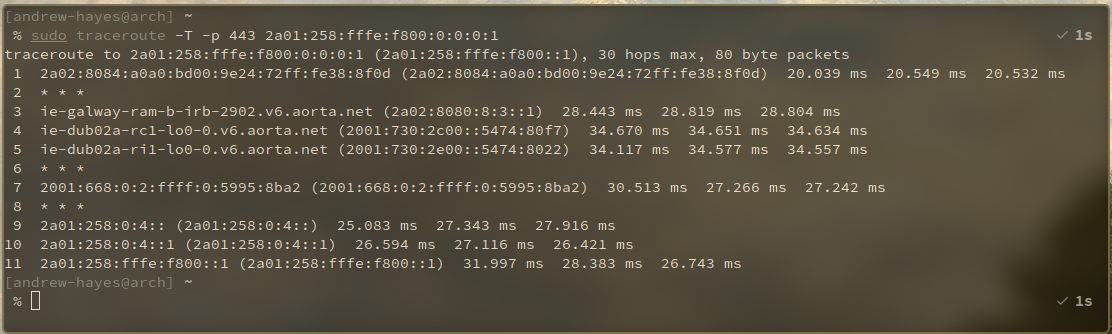
\includegraphics[width=\textwidth]{./images/irelandtraceroute.png}
    \caption{Output of \texttt{sudo traceroute -T -p 443 2a01:258:fffe:f800:0:0:0:1}}
\end{figure}

\subsection{UK Server}
The UK server I added had \verb|remote| \verb|213.5.132.231|.

\begin{figure}[H]
    \centering
    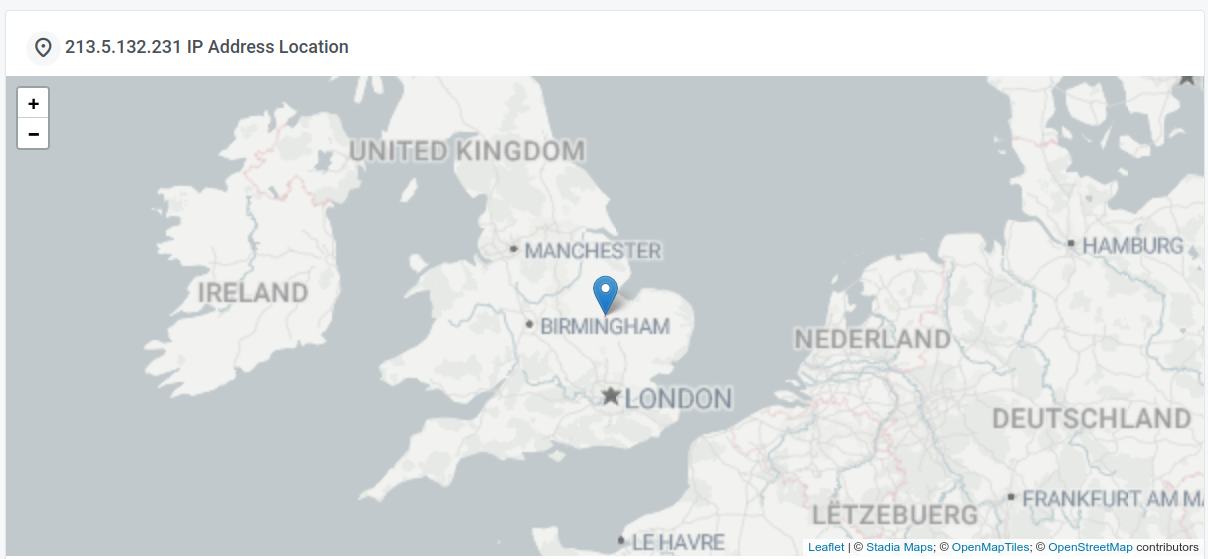
\includegraphics[width=\textwidth]{./images/ukserverloc.png}
    \caption{Location of my chosen UK server (source: \url{https://www.ipaddress.com/})}
\end{figure}

According to \url{https://gps-coordinates.org/distance-between-coordinates.php} the distance between the latitude and longitude of Galway (as given in the assignment specification) and the United Kingdom server is 595.76 kilometres.
The server also seemed to be blocking ICMPv6 packets sent via \verb|traceroute|, so I instead used \mintinline{shell}{sudo traceroute -T -p 443} to send TCP packets to circumvent this.
The number of hops to the destination server was 12.

\begin{figure}[H]
    \centering
    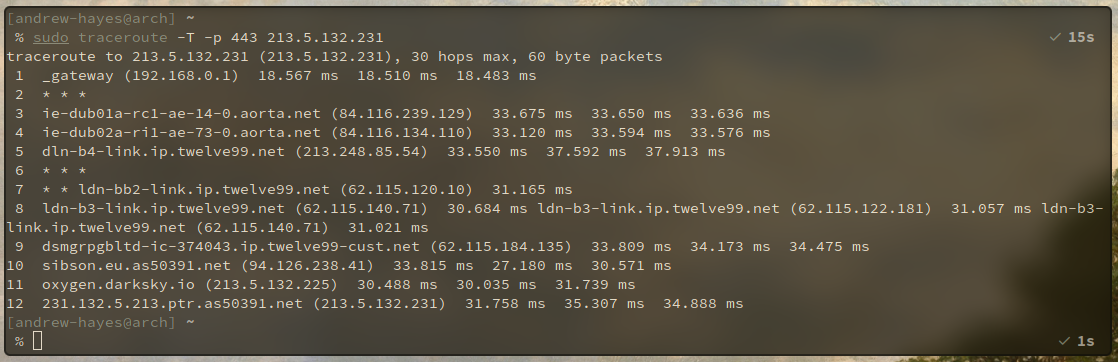
\includegraphics[width=\textwidth]{./images/uktraceroute.png}
    \caption{Output of \texttt{sudo traceroute -T -p 443 213.5.132.231}}
\end{figure}

\subsection{Europe Server}
The Europe server I added had \verb|remote| \verb|150.241.82.187|.

\begin{figure}[H]
    \centering
    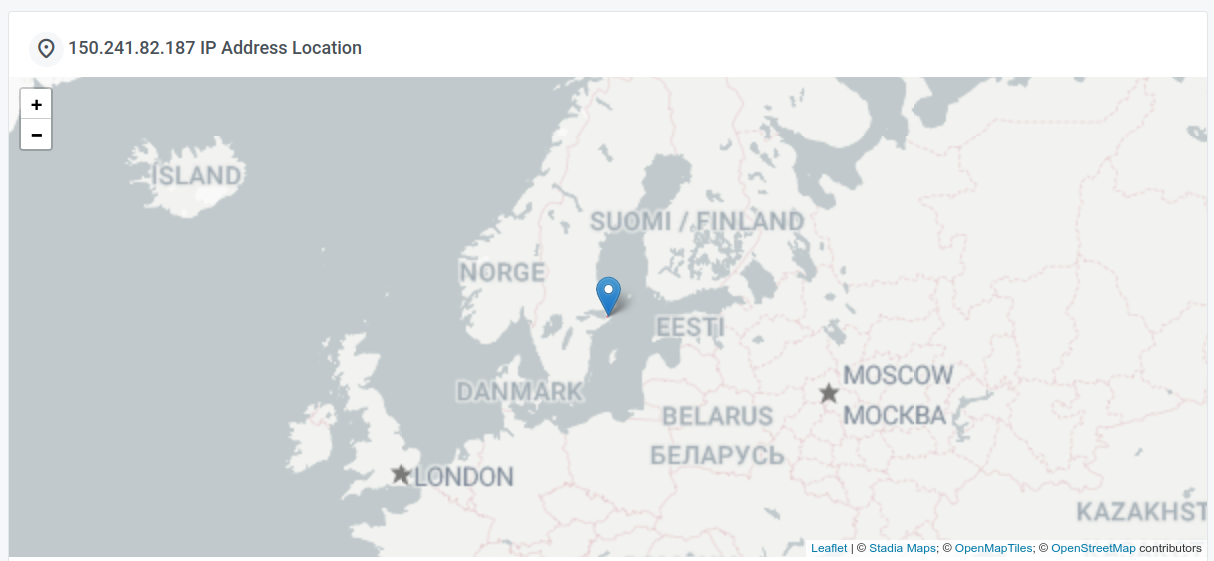
\includegraphics[width=\textwidth]{./images/europeserverloc.png}
    \caption{Location of my chosen Europe server (source: \url{https://www.ipaddress.com/})}
\end{figure}

According to \url{https://gps-coordinates.org/distance-between-coordinates.php} the distance between the latitude and longitude of Galway (as given in the assignment specification) and the Europe Server is 1788.51 kilometres.
The number of hops to the destination server was 14.

\begin{figure}[H]
    \centering
    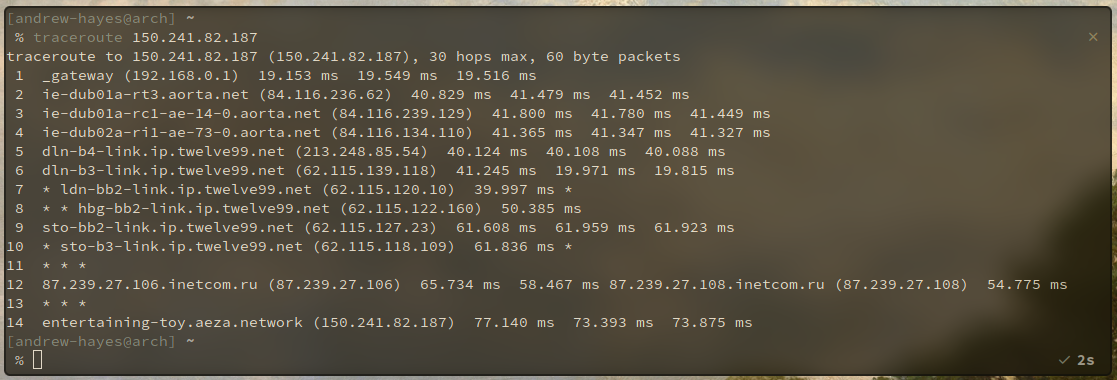
\includegraphics[width=\textwidth]{./images/europetraceroute.png}
    \caption{Output of \texttt{traceroute 150.241.82.187}}
\end{figure}

\subsection{United States Server}
The United States server I added had \verb|remote| \verb|arm1.maxhost.io| and appeared in the \mintinline{shell}{ntpq -p} output with \verb|remote| \verb|2603:c020:0:836| which is an abbreviated for of the IPv6 address \verb|2603:c020:0000:0836::|.

\begin{figure}[H]
    \centering
    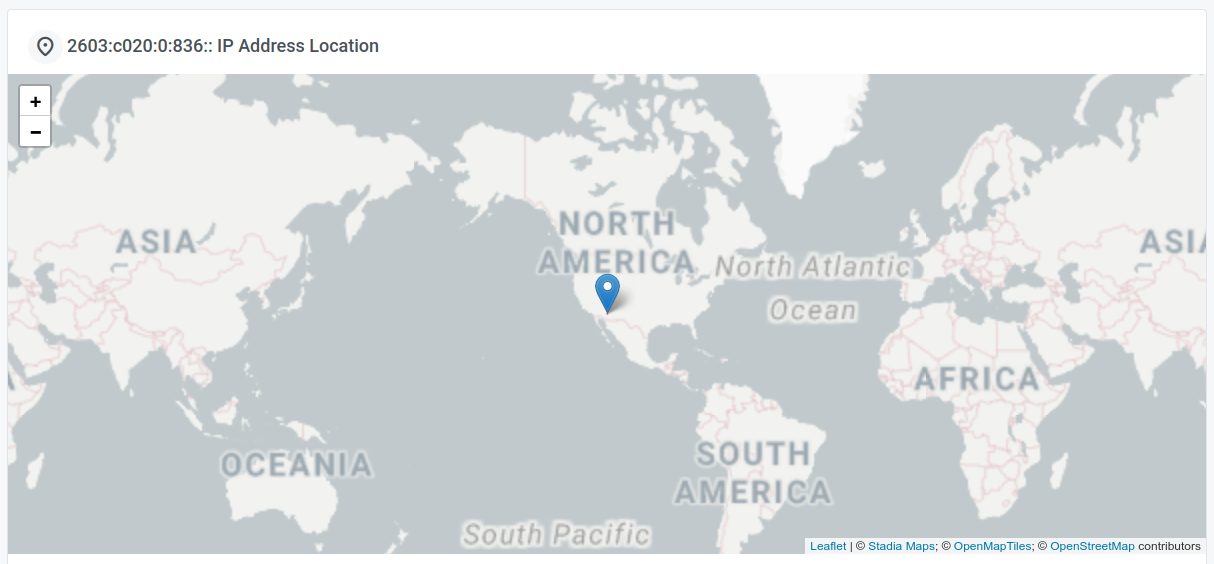
\includegraphics[width=\textwidth]{./images/usserverloc.png}
    \caption{Location of my chosen United States server (source: \url{https://www.ipaddress.com/})}
\end{figure}

According to \url{https://gps-coordinates.org/distance-between-coordinates.php} the distance between the latitude and longitude of Galway (as given in the assignment specification) and the United States server is 7863.25 kilometres.
The server seemed to be blocking both ICMPv6 and TCP packets sent via \mintinline{shell}{traceroute}.
As a final attempt, I tried to pretend to be an NTP packet by pinging the well-known NTP port \verb|123| with UDP packets but that didn't work.
In each attempt, the \mintinline{shell}{traceroute} stopped making progress at the 9\textsuperscript{th} hop, so I'm guessing that the 10\textsuperscript{th} hop might be the server itself had the \mintinline{shell}{traceroute} gone through.

\begin{figure}[H]
    \centering
    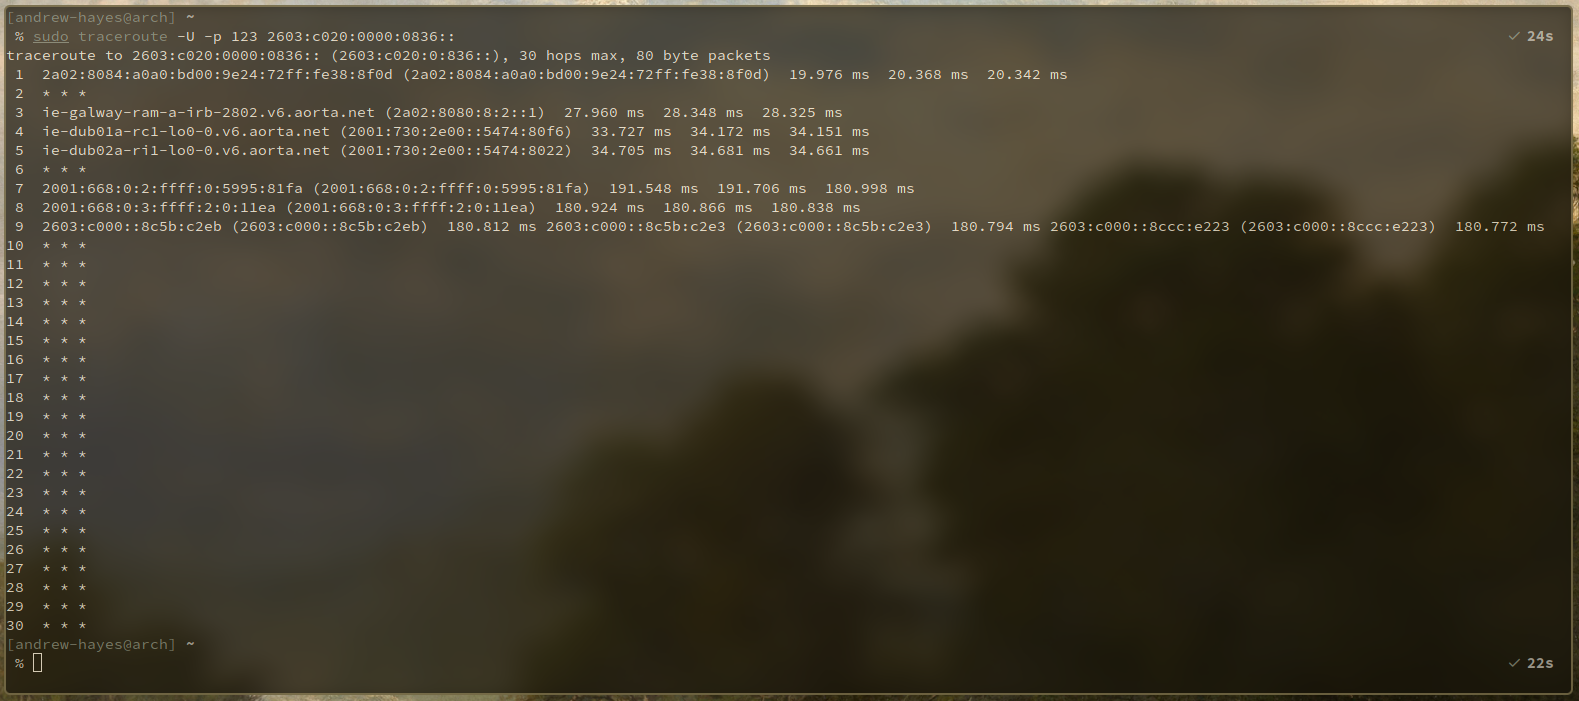
\includegraphics[width=\textwidth]{./images/ustraceroute.png}
    \caption{Output of \texttt{sudo traceroute -U -p 123 2603:c020:0000:0836::}}
\end{figure}

\subsection{Australia Server}
The Australia server I added had \verb|remote| \verb|159.196.178.7|.

\begin{figure}[H]
    \centering
    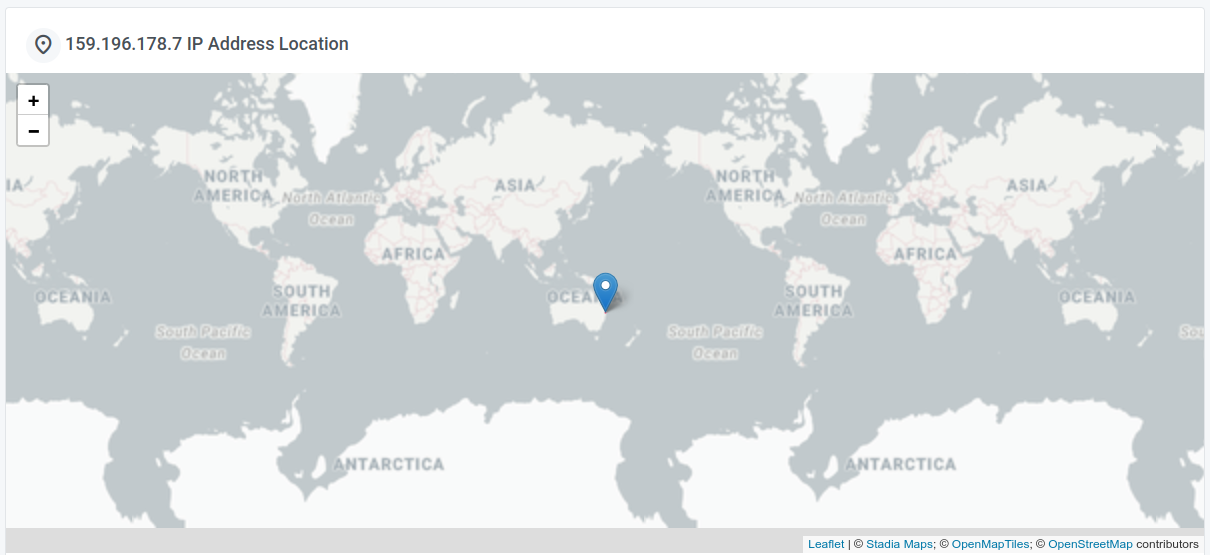
\includegraphics[width=\textwidth]{./images/australiaserverloc.png}
    \caption{Location of my chosen Australia server (source: \url{https://www.ipaddress.com/})}
\end{figure}

According to \url{https://gps-coordinates.org/distance-between-coordinates.php} the distance between the latitude and longitude of Galway (as given in the assignment specification) and the Australia server is 16790.45 kilometres.
The server also seemed to be blocking ICMPv6 packets sent via \mintinline{shell}{traceroute}, so I instead used \mintinline{shell}{sudo traceroute -T -p 443} to send TCP packets to circumvent this.
The number of hops to the destination server was 15.

\begin{figure}[H]
    \centering
    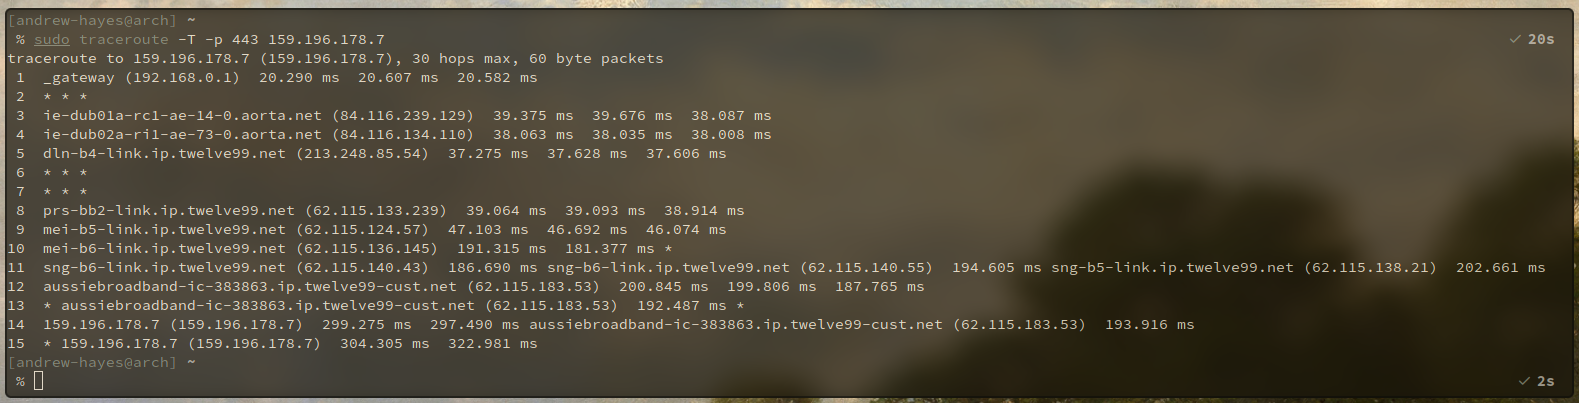
\includegraphics[width=\textwidth]{./images/australiatraceroute.png}
    \caption{Output of \texttt{sudo traceroute -T -p 443 159.196.178.7}}
\end{figure}

\subsection{Asia Server}
The Asia server I added had \verb|remote| \verb|202.65.114.202|.

\begin{figure}[H]
    \centering
    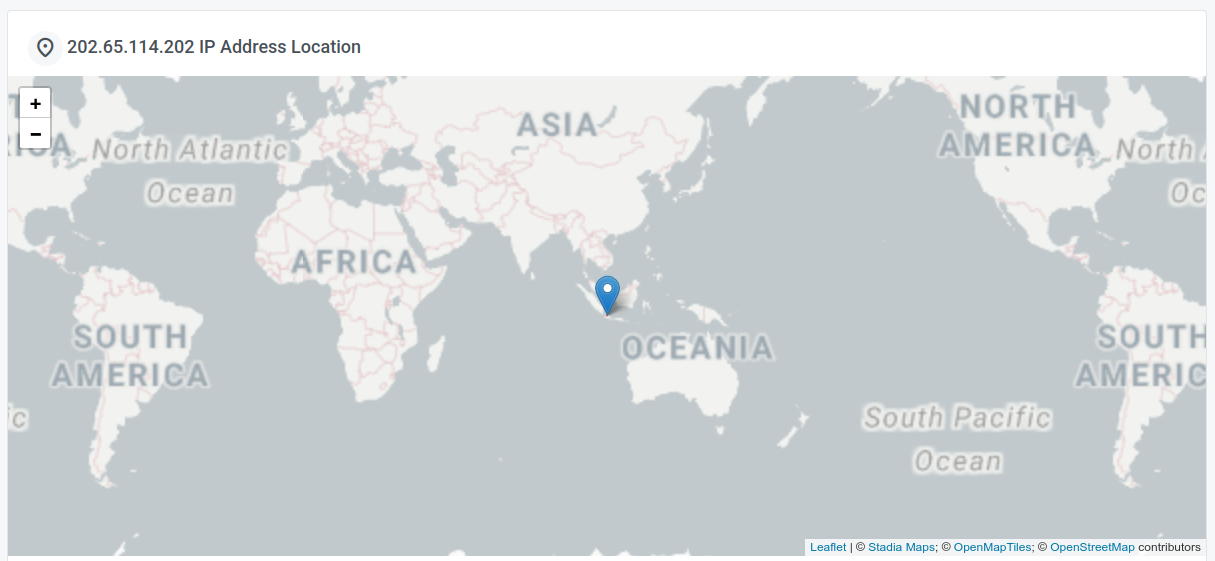
\includegraphics[width=\textwidth]{./images/asiaserverloc.png}
    \caption{Location of my chosen Asia server (source: \url{https://www.ipaddress.com/})}
\end{figure}

According to \url{https://gps-coordinates.org/distance-between-coordinates.php} the distance between the latitude and longitude of Galway (as given in the assignment specification) and the Asia Server is 12256.96 kilometres.
The number of hops to the destination server was 14.

\begin{figure}[H]
    \centering
    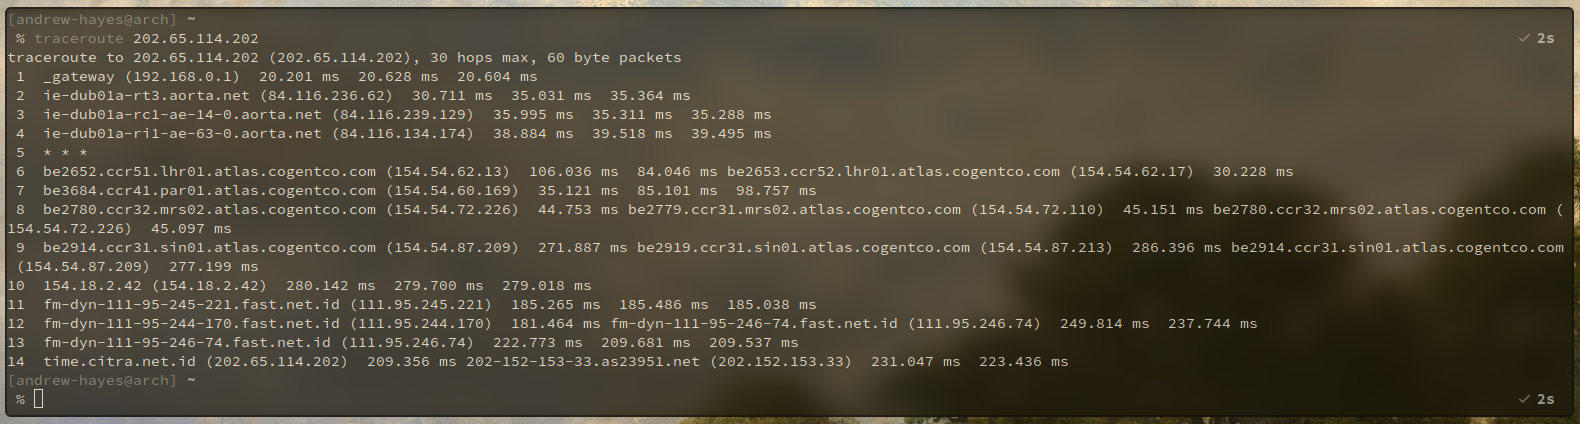
\includegraphics[width=\textwidth]{./images/asiatraceroute.png}
    \caption{Output of \texttt{traceroute 202.65.114.202}}
\end{figure}

\section{Collected Data}
I collected the NTP peers data over a period of 8 hours with one query every 20 minutes using a shell script which would then parse the data into TSV (tab-separated value) format and append it to a file called \verb|results.tsv|.

\begin{code}
\inputminted[texcl, mathescape, linenos, breaklines, frame=single]{shell}{../code/query.sh}
\caption{\texttt{query.sh}}
\end{code}

The \verb|remote| column for the UK server contained a single \verb|(| character in the output, the meaning of which I'm not quite sure as I couldn't find anything about it in the NTP documentation or manual pages, which made parsing the data more difficult so I just removed any instances of the character from the file using the command \mintinline{shell}{sed -i 's/\(\t//g' results.tsv}.
Then, I removed the prefix characters (\verb|+|, \verb|-|, \verb|*|) from the \verb|remote| column using Vim with visual-block editing.
Finally, I wrote a short Python script to ingest the data, plot it, and perform the necessary calculations.

\begin{table}[H]
    \centering
    \begin{tabular}{lcccc}
        \hline
        Server & Max & Min & Mean & Std \\ 
        \hline
        Asia       & 36.340 & 1.538 & 14.799 & 14.314 \\
        Australia  & 38.036 & 2.142 & 20.088 & 12.054 \\
        Europe     & 31.494 & 0.735 & 5.296  & 6.040  \\
        Ireland    & 32.574 & 0.882 & 12.049 & 12.067 \\
        UK         & 48.932 & 0.587 & 6.474  & 9.322  \\
        US         & 40.647 & 0.434 & 6.249  & 8.860  \\
        \hline
    \end{tabular}
    \caption{Jitter statistics}
\end{table}

\begin{table}[H]
    \centering
    \begin{tabular}{lcccc}
        \hline
        Server & Max & Min & Mean & Std \\ 
        \hline
        Asia       & 222.677 & 207.773 & 213.492 & 4.114 \\
        Australia  & 335.595 & 295.743 & 308.813 & 10.419 \\
        Europe     & 79.569  & 57.901  & 67.093  & 6.319  \\
        Ireland    & 41.311  & 22.422  & 28.672  & 5.045  \\
        UK         & 46.231  & 28.801  & 34.843  & 5.228  \\
        US         & 201.211 & 180.389 & 186.829 & 5.196  \\
        \hline
    \end{tabular}
    \caption{Delay statistics}
\end{table}

\begin{table}[H]
    \centering
    \begin{tabular}{lcccc}
        \hline
        Server & Max & Min & Mean & Std \\ 
        \hline
        Asia       & 6.475  & -10.676 & -5.678  & 3.500  \\
        Australia  & -1.570 & -31.768 & -17.999 & 5.977  \\
        Europe     & 46.757 & -7.301  & 0.464   & 10.393 \\
        Ireland    & 8.914  & -2.956  & 2.186   & 4.099  \\
        UK         & 5.197  & -14.073 & -1.955  & 4.641  \\
        US         & -7.888 & -24.577 & -18.804 & 4.837  \\
        \hline
    \end{tabular}
    \caption{Offset statistics}
\end{table}

I think that the results indicate a strong correlation between delay, jitter, \& offset with geographical distance and number of packet hops.
As we saw previously, the number of packet hops was higher the further away the server was geographically from my computer.
The Irish server needed only 11 hops, the UK server 12, the European server 14, the Australian server 15, and the Asian server 14.
We estimated that the American server could've been accessed in just 10 hops, but really there's no good way of knowing since the packet was blocked every time.
This pattern continues with the jitter, delay, and offset statistics:
looking at the mean column for each table above, the Australian and US servers consistently have the highest absolute value, being the furthest away geographically.
This is to be expected, as the packets have to take more time to physically travel across the world to those locations.
Interestingly, the Irish server has consistently high jitter: one key reason for this might be that the data was collected across afternoon and evening time in Ireland, which are likely to peak times for load on Irish NTP servers and therefore introduce more jitter.
Another interesting observation is that the Irish mean offset is actually more than the European mean offset; however, I think this can be explained by the fact that European offset had a much higher standard deviation, and a much wider range of offset values, which average out to be closer to zero despite being significantly worse.

\begin{figure}[H]
    \centering
    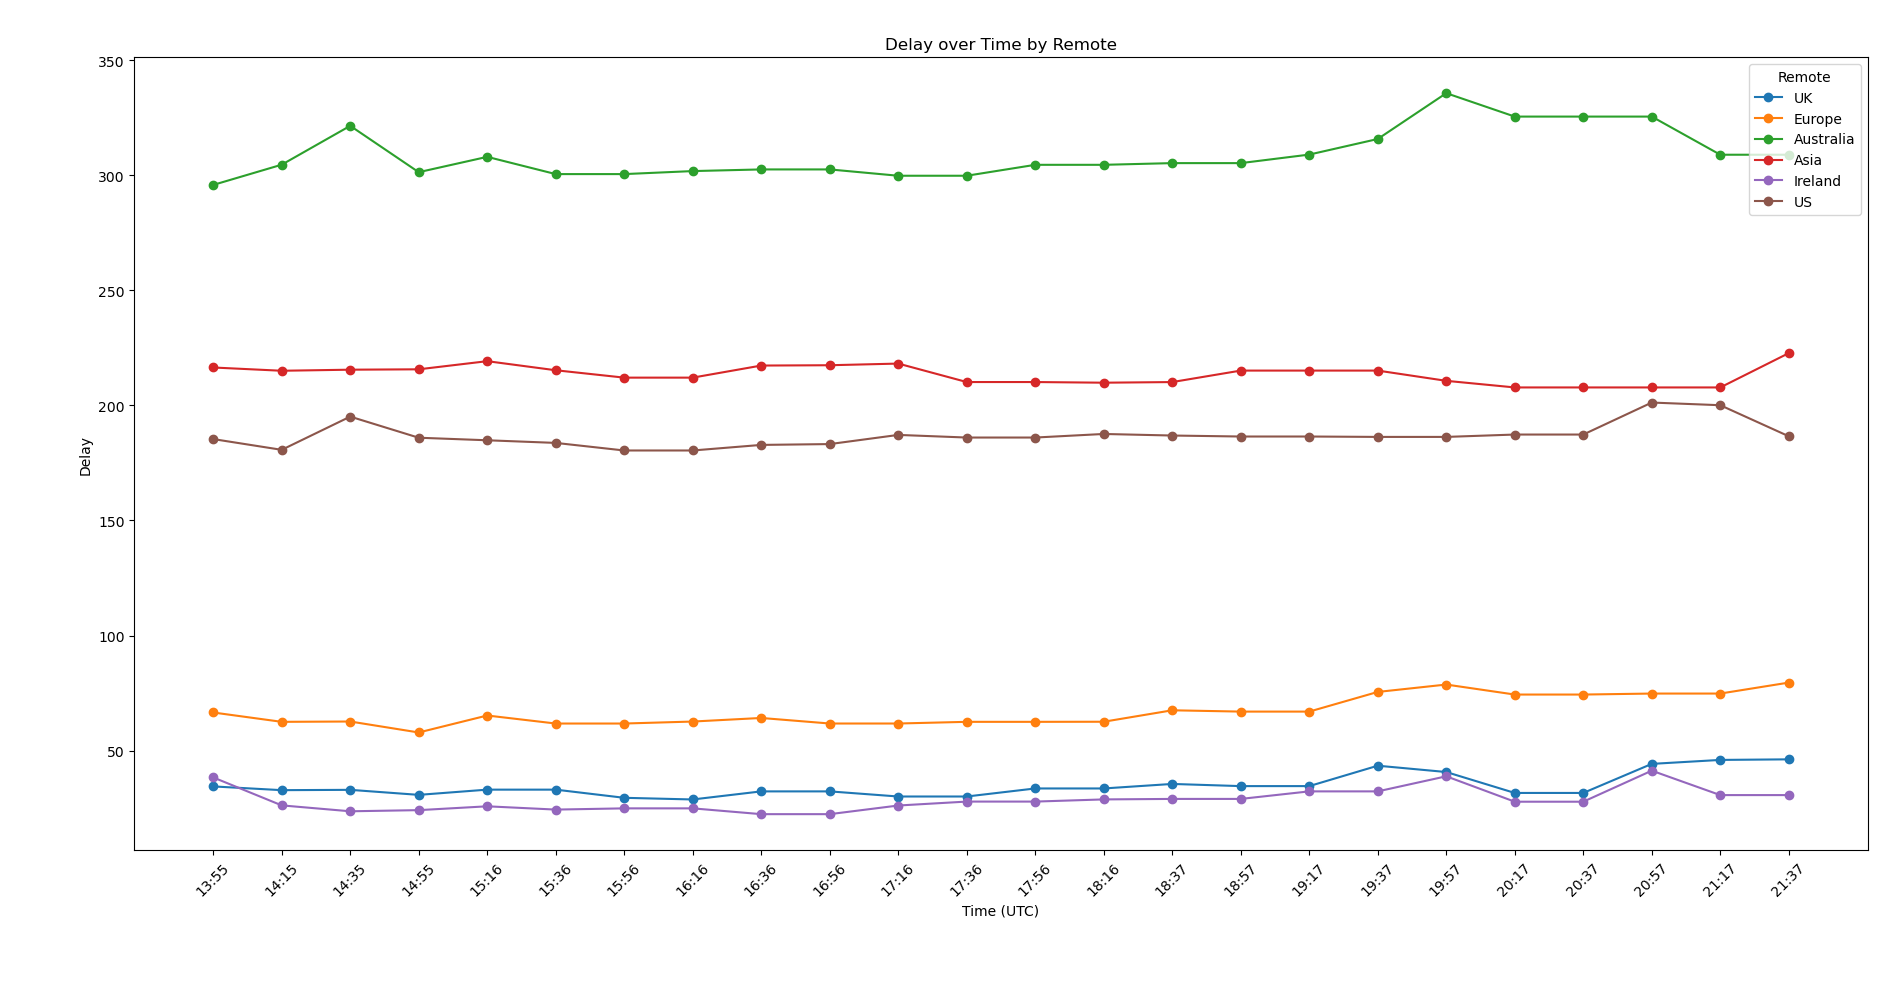
\includegraphics[width=\textwidth]{./images/delayplot.png}
    \caption{Delay over Time}
\end{figure}

The results of plotting delay against time are exactly as one would expect:
the further away a server is, the higher the offset.
Asutralia has consistently the highest offset, followed by Asia, followed by US, followed by Europe, UK, \& Ireland.
We can see that the Irish server's delay follows the UK's server delay very closely:
this is likely due to the closeness in time zones -- both servers would face peak hours at roughly the same times.
The delay for these servers peaks in the evening time, when people are off work and home from school and thus using Internet-connected devices.
However, for the most part, even with the temporal variation in the delay values, they stay remarkably consistent, which indicates that while they are somewhat dependent on the time of day, the delay values are primarily determined by geographical distance.

\begin{figure}[H]
    \centering
    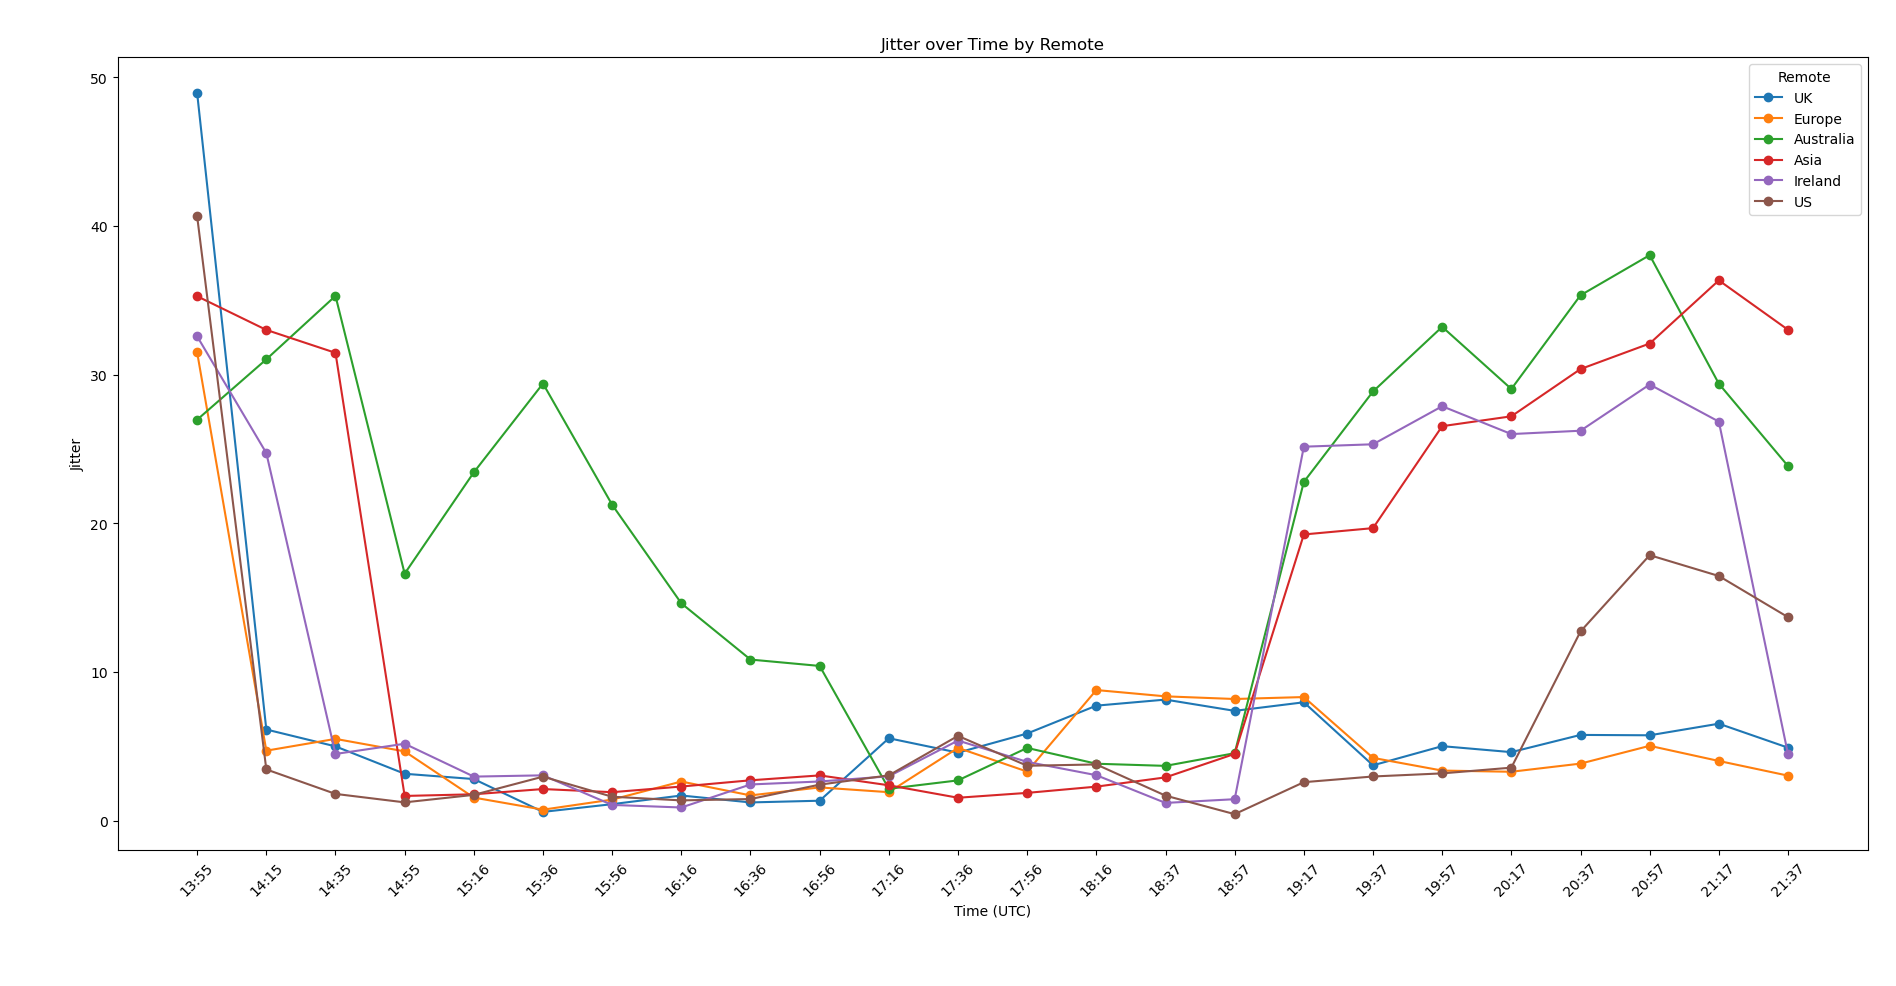
\includegraphics[width=\textwidth]{./images/jitterplot.png}
    \caption{Jitter over Time}
\end{figure}

The jitter over time varies a great deal more.
Of course, since jitter is a measure of the variance in delay, we can see that the jitter values peak for around the same times that there are small peaks in the delay data.
Again, the Irish server's jitter peaks in the evening time, as one would expect.
We can also see that despite varying more than the offset, the jitter values across different servers seem to be more aligned, being low around the same times and high around the same times, giving strong evidence that jitter is influenced by the time of day.

\begin{figure}[H]
    \centering
    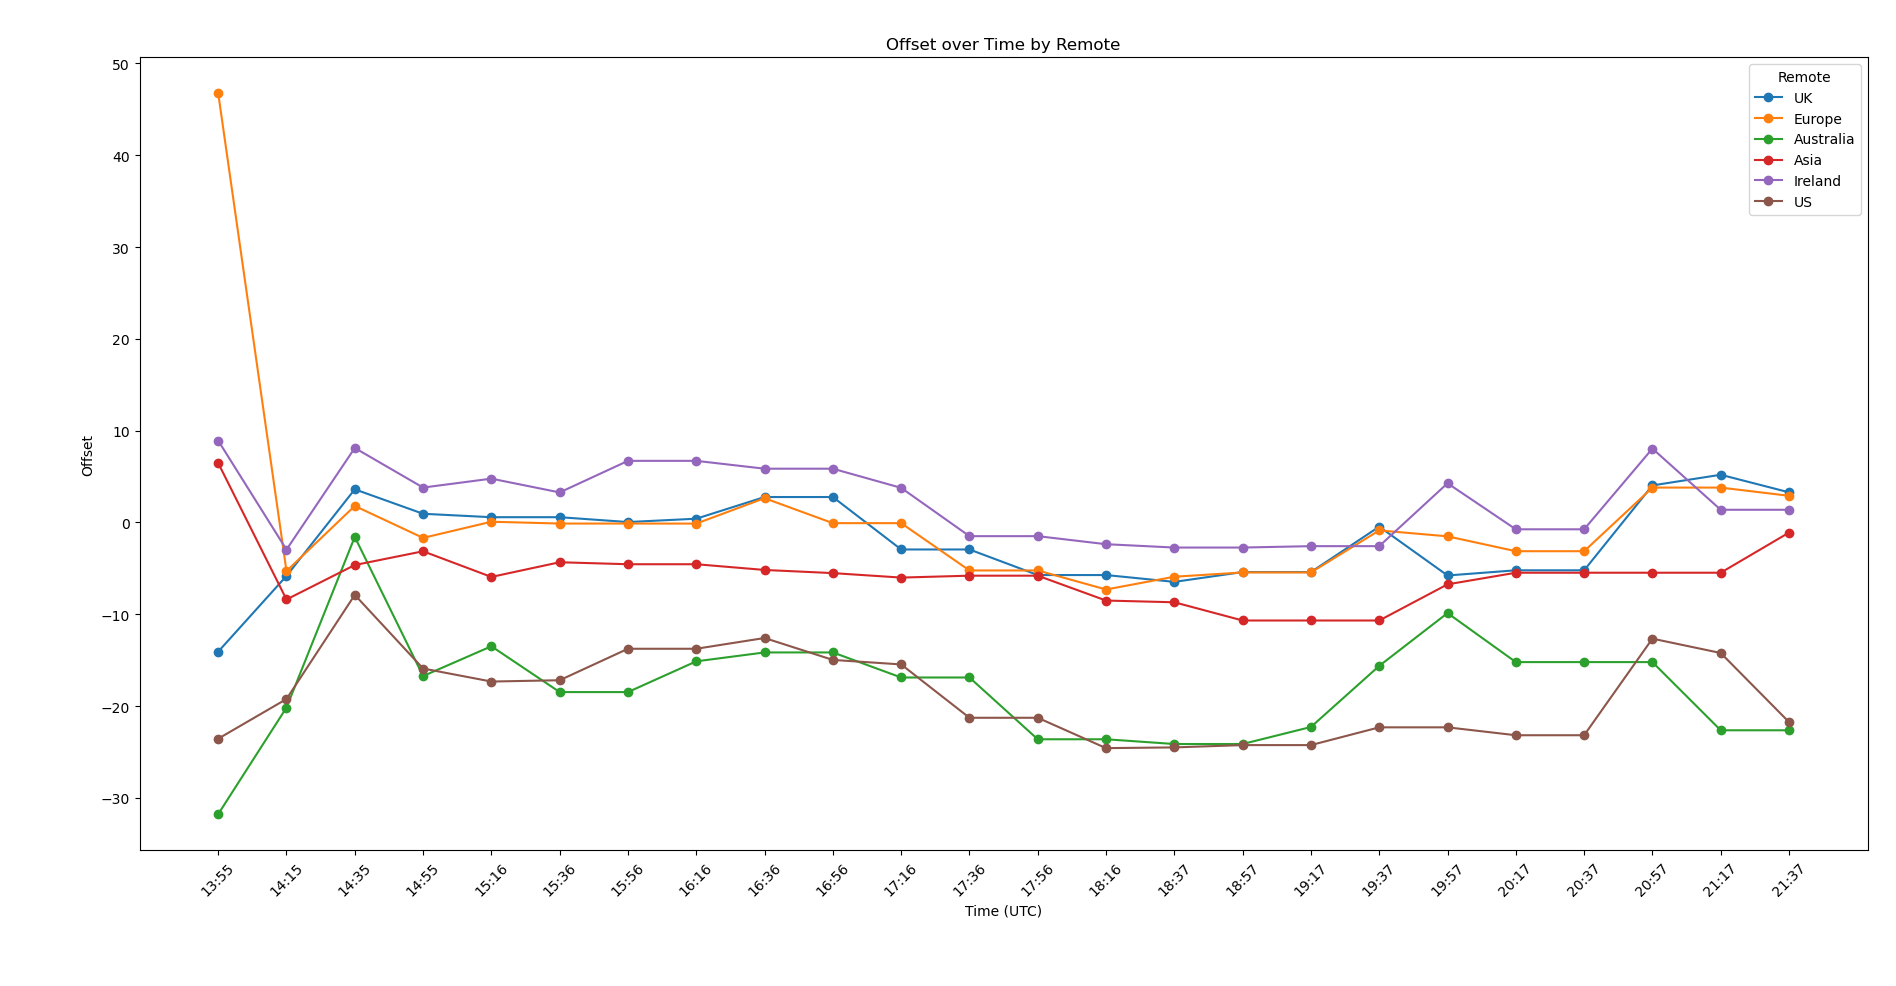
\includegraphics[width=\textwidth]{./images/offsetplot.png}
    \caption{Offset over Time}
\end{figure}

We can see that offset also varies over time, more wildly than the delay but less so than the jitter.
We can also see that despite offset varying less than jitter, the offset curves tend to go up when the jitter curves go up, which makes sense, as greater variance and inconsistency in the amount of time a packet takes to get to its destination will necessarily impact the offset.



\end{document}
